\documentclass[aspectratio=169,10pt]{beamer}

% ---- Packages ----------------------------------------------------------
\usepackage[T1]{fontenc}
\usepackage{lmodern}
\usepackage{microtype}
\usepackage{booktabs}
\usepackage{array}
\usepackage{multirow}
\usepackage{graphicx}
\usepackage{tikz}
\usepackage{xcolor}
\usepackage{amsmath}
\usepackage{calc}

\graphicspath{{figures/}}

% ---- Brand palette -----------------------------------------------------
\definecolor{garnet}{HTML}{73000A}
\definecolor{rose}{HTML}{CC2E40}
\definecolor{atlantic}{HTML}{466A9F}
\definecolor{congaree}{HTML}{1F414D}
\definecolor{horseshoe}{HTML}{65780B}
\definecolor{honeycomb}{HTML}{A49137}
\definecolor{warmgrey}{HTML}{676156}
\definecolor{sandstorm}{HTML}{FFF2E3}
\definecolor{black90}{HTML}{363636}
\definecolor{black70}{HTML}{5C5C5C}
\definecolor{black50}{HTML}{A2A2A2}
\definecolor{black30}{HTML}{C7C7C7}
\definecolor{black10}{HTML}{ECECEC}

% ---- Theme: minimal, no rounded edges ----------------------------------
\usetheme{default}
\useinnertheme{rectangles}
\useoutertheme{default}
\beamertemplatenavigationsymbolsempty
\setbeamertemplate{itemize items}[square]
\setbeamertemplate{enumerate items}[default]

\setbeamercolor{structure}{fg=garnet}
\setbeamercolor{title}{fg=garnet}
\setbeamercolor{frametitle}{fg=black, bg=white}
\setbeamercolor{normal text}{fg=black90}
\setbeamercolor{alerted text}{fg=garnet}
\setbeamercolor{itemize item}{fg=garnet}
\setbeamercolor{itemize subitem}{fg=black70}
\setbeamercolor{block title}{fg=white, bg=garnet}
\setbeamercolor{block body}{fg=black90, bg=black10}
\setbeamercolor{caption name}{fg=garnet}
\setbeamercolor{footline}{fg=black70, bg=white}
\setbeamerfont{frametitle}{size=\large,series=\bfseries}
\setbeamerfont{footline}{size=\tiny}

% Flat blocks (no rounded corners)
\setbeamertemplate{blocks}[default]

% Custom frametitle: garnet rule under title
\setbeamertemplate{frametitle}{%
  \nointerlineskip
  \vskip0.35em
  \begin{beamercolorbox}[wd=\paperwidth,leftskip=0.9em,rightskip=0.9em]{frametitle}
    \usebeamerfont{frametitle}\insertframetitle\par
    \vskip2pt
    {\color{garnet}\rule{\dimexpr\paperwidth-1.8em\relax}{1.2pt}}
  \end{beamercolorbox}
  \vskip0.4em
}

% Footline: author | title | slide number
\setbeamertemplate{footline}{%
  \hbox{%
    \begin{beamercolorbox}[wd=\paperwidth,ht=2.2ex,dp=1ex,leftskip=1em,rightskip=1em]{footline}
      \usebeamerfont{footline}%
      Vaught \& Dangerfield \hfill CSCE~763 \hfill \insertframenumber/\inserttotalframenumber
    \end{beamercolorbox}%
  }%
}

% ---- Metadata ----------------------------------------------------------
\title{Classical vs.\ Deep Learning Object Detection\\ in X-Band Marine Radar Imagery}
\author{J.C.\ Vaught \and Ty Dangerfield}
\institute{University of South Carolina \textbullet{} CSCE~763}
\date{April 2026}

% ---- Convenience macros ------------------------------------------------
\newcommand{\hl}[1]{\textcolor{garnet}{\textbf{#1}}}
\newcommand{\sub}[1]{{\footnotesize\textcolor{black70}{#1}}}

\begin{document}

% =======================================================================
% 1 Title
% =======================================================================
\begin{frame}[plain]
  \vspace{0.4em}
  {\color{garnet}\rule{\textwidth}{1.4pt}}\par\vspace{0.6em}
  {\Large\bfseries\color{black90} Classical vs.\ Deep Learning Object Detection\\ in X-Band Marine Radar Imagery\par}
  \vspace{0.8em}
  {\large J.C.\ Vaught \quad\textbullet\quad Ty Dangerfield\par}
  \vspace{0.2em}
  {\color{black70}University of South Carolina~~\textbullet~~CSCE~763 Final Project\par}
  \vspace{0.4em}
  {\color{garnet}\rule{\textwidth}{0.8pt}}\par
  \vfill
  \begin{columns}[T,onlytextwidth]
    \column{0.58\textwidth}
      \footnotesize\color{black70}
      First cross-paradigm benchmark of 7~classical + 4~deep detectors\\
      on the DLR DAAN / DARC / MANV corpus, under a single
      AIS-anchored ground truth with per-dataset polar calibration.
    \column{0.38\textwidth}
      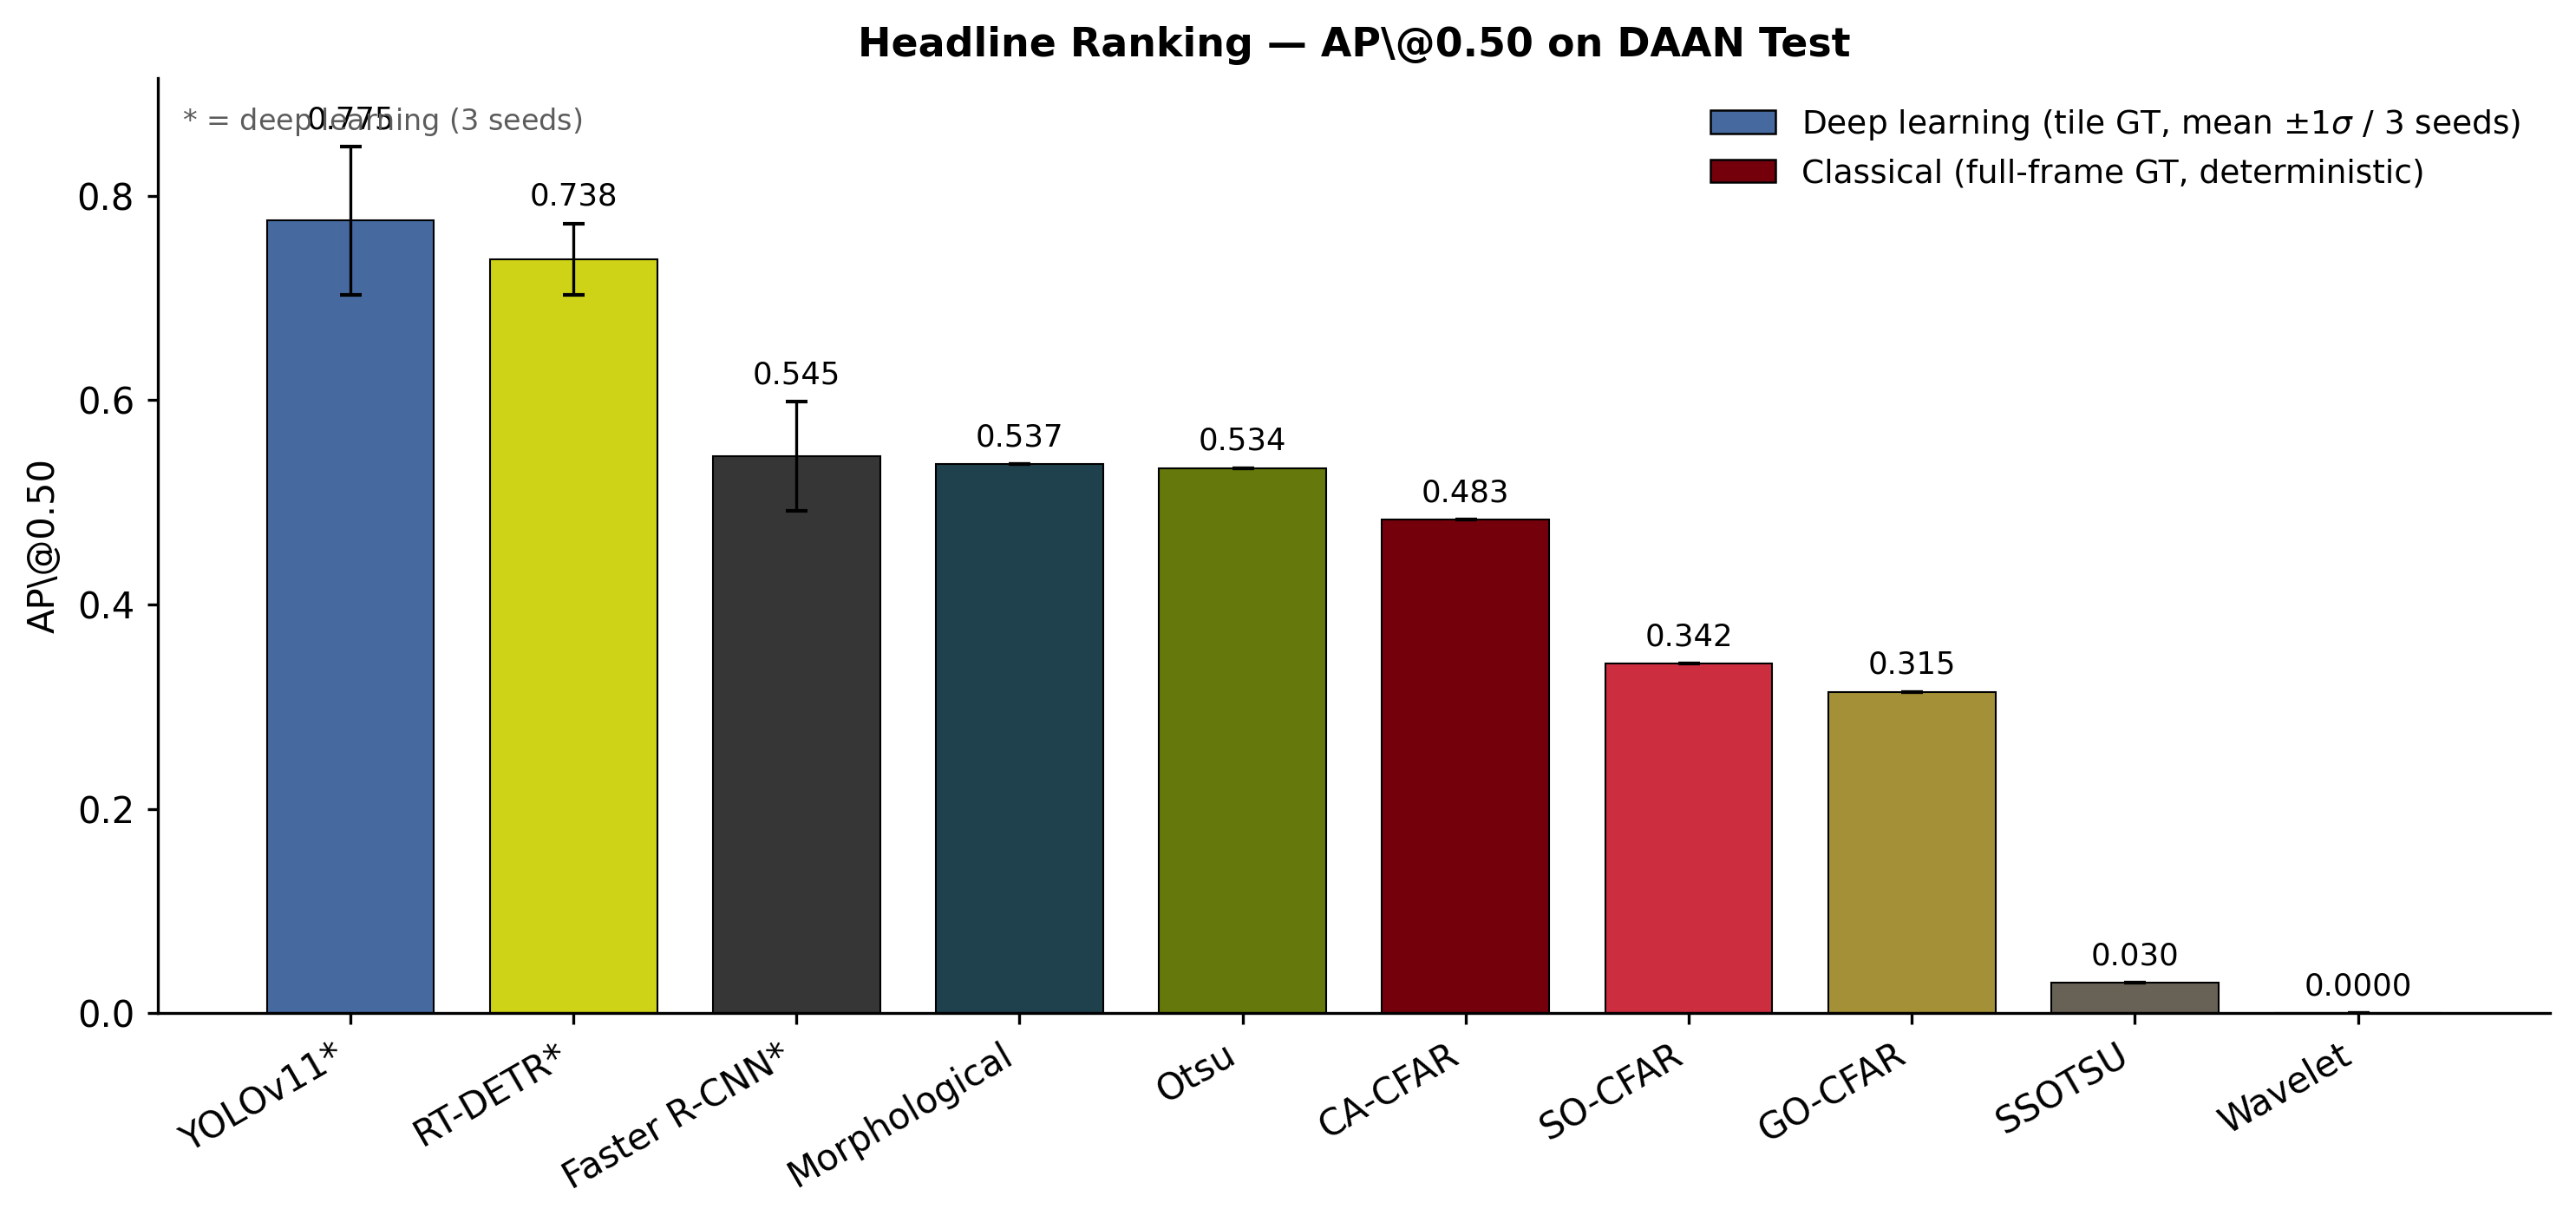
\includegraphics[width=\linewidth]{fig1_headline.png}
  \end{columns}
  \vspace{0.6em}
  {\tiny\color{black70}April 2026}
\end{frame}

% =======================================================================
% 2 Motivation
% =======================================================================
\begin{frame}{Why marine radar detection?}
  \begin{columns}[T,onlytextwidth]
    \column{0.58\textwidth}
      \begin{itemize}\setlength\itemsep{0.5em}
        \item X-band marine radar produces \hl{plan-position-indicator (PPI)} imagery.
        \item Vessels, buoys, and debris appear as bright returns over sea clutter.
        \item Core problem for \hl{maritime safety} and \hl{autonomous surface vehicles}.
        \item Detection pipelines historically split into two camps:
          \begin{itemize}\setlength\itemsep{0.2em}
            \item[\textcolor{garnet}{$\blacksquare$}] Classical signal/image processing (CFAR, morphology, wavelets, Otsu).
            \item[\textcolor{atlantic}{$\blacksquare$}] Modern deep detectors (YOLO, DETR, Faster R-CNN, U-Net).
          \end{itemize}
      \end{itemize}
    \column{0.38\textwidth}
      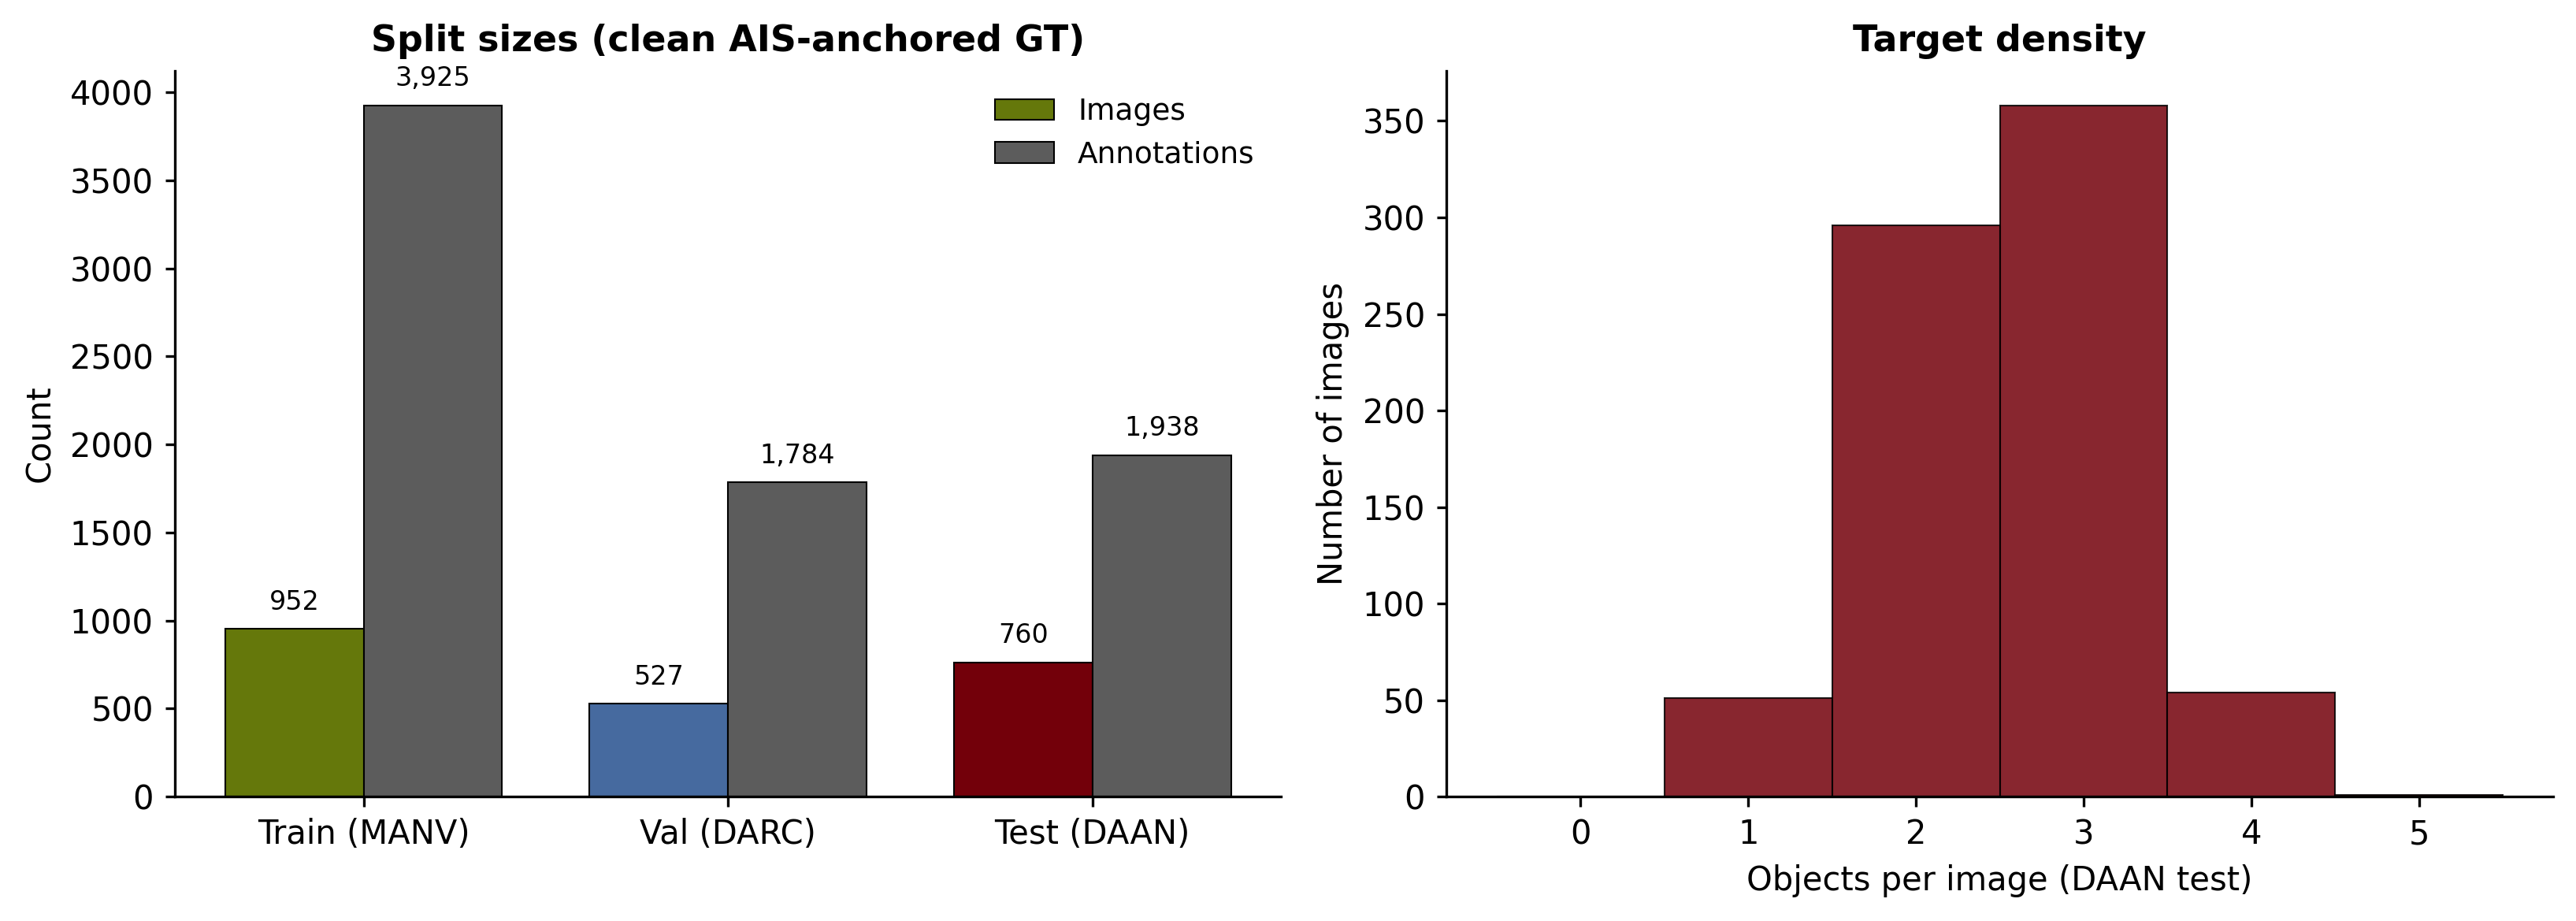
\includegraphics[width=\linewidth]{fig8_dataset.png}\par
      \sub{DLR corpus at a glance: per-sub-dataset split sizes and target-density distribution across the 2{,}239 evaluated frames.}
  \end{columns}
\end{frame}

% =======================================================================
% 3 Gap and question
% =======================================================================
\begin{frame}{The gap in the literature}
  \begin{itemize}\setlength\itemsep{0.55em}
    \item Recent DL results on marine radar look spectacular:\\
          YOLOv11 \hl{mAP@0.5 $>$ 0.95}~[Heuer 2025]; Marine-Faster R-CNN \hl{93.6\%} recall~[Chen 2022].
    \item Classical methods (CA/GO/SO/OS-CFAR, SWT, Otsu) have \hl{decades} of theory but sparse modern reporting.
    \item \alert{No single study} evaluates both paradigms on \hl{identical data, identical GT, and identical metrics}.
  \end{itemize}
  \vspace{0.6em}
  \begin{block}{Research question}
    On a shared X-band PPI benchmark, how large is the classical-vs-deep gap when every detector is evaluated
    under the same AIS-anchored ground truth and the same COCO protocol?
  \end{block}
\end{frame}

% =======================================================================
% 4 Methods overview
% =======================================================================
\begin{frame}{Eleven detectors, two paradigms}
  \centering
  \footnotesize
  \renewcommand{\arraystretch}{1.05}
  \begin{tabular}{@{}>{\raggedright\arraybackslash}p{0.17\textwidth}
                     >{\raggedright\arraybackslash}p{0.29\textwidth}
                     >{\raggedright\arraybackslash}p{0.45\textwidth}@{}}
    \toprule
    \textbf{Family} & \textbf{Method} & \textbf{Core idea} \\
    \midrule
    \multirow{3}{*}{\textcolor{garnet}{Classical CFAR}}
      & CA-CFAR & Cell-averaged adaptive threshold \\
      & GO-CFAR / SO-CFAR & Greatest-of / smallest-of leading \& lagging cells \\
      & OS-CFAR & Order-statistic (rank-based) threshold \\
    \midrule
    \multirow{3}{*}{\textcolor{garnet}{Other classical}}
      & Morphological & Otsu $\rightarrow$ opening $\rightarrow$ connected components \\
      & Wavelet (SWT) & 2-D stationary wavelet high-freq.\ sub-band threshold \\
      & SSOTSU & Seed-point Otsu for small-target segmentation \\
    \midrule
    \multirow{4}{*}{\textcolor{atlantic}{Deep learning}}
      & YOLOv11 (with SAHI) & 1-stage anchor-free, tiled inference \\
      & RT-DETR & Transformer end-to-end, NMS-free \\
      & Faster R-CNN & 2-stage anchor-optimised for radar \\
      & U-Net & Per-pixel segmentation $\rightarrow$ bbox \\
    \bottomrule
  \end{tabular}
  \vspace{0.4em}
  \par\sub{All detectors receive identical preprocessed PPI input and emit COCO-format boxes for unified evaluation.}
\end{frame}

% =======================================================================
% 5 Dataset
% =======================================================================
\begin{frame}{Dataset: DLR DAAN / DARC / MANV}
  \begin{columns}[T,onlytextwidth]
    \column{0.52\textwidth}
      \begin{itemize}\setlength\itemsep{0.45em}
        \item \hl{DLR open marine radar corpus} --- three sub-datasets:
          \begin{itemize}\setlength\itemsep{0.15em}
            \item \textbf{MANV} --- harbour manoeuvres, \hl{6\,m/px}, close-range.
            \item \textbf{DARC} --- open water, \hl{12\,m/px}.
            \item \textbf{DAAN} --- open water, \hl{12\,m/px}.
          \end{itemize}
        \item \textbf{2{,}239} PPI frames and \textbf{11{,}893} target instances total.
        \item Annotations include \hl{AIS transponder track}, bounding boxes, and segmentation.
        \item Split (paper convention): MANV $\rightarrow$ train, DARC $\rightarrow$ val, DAAN $\rightarrow$ test.
      \end{itemize}
    \column{0.44\textwidth}
      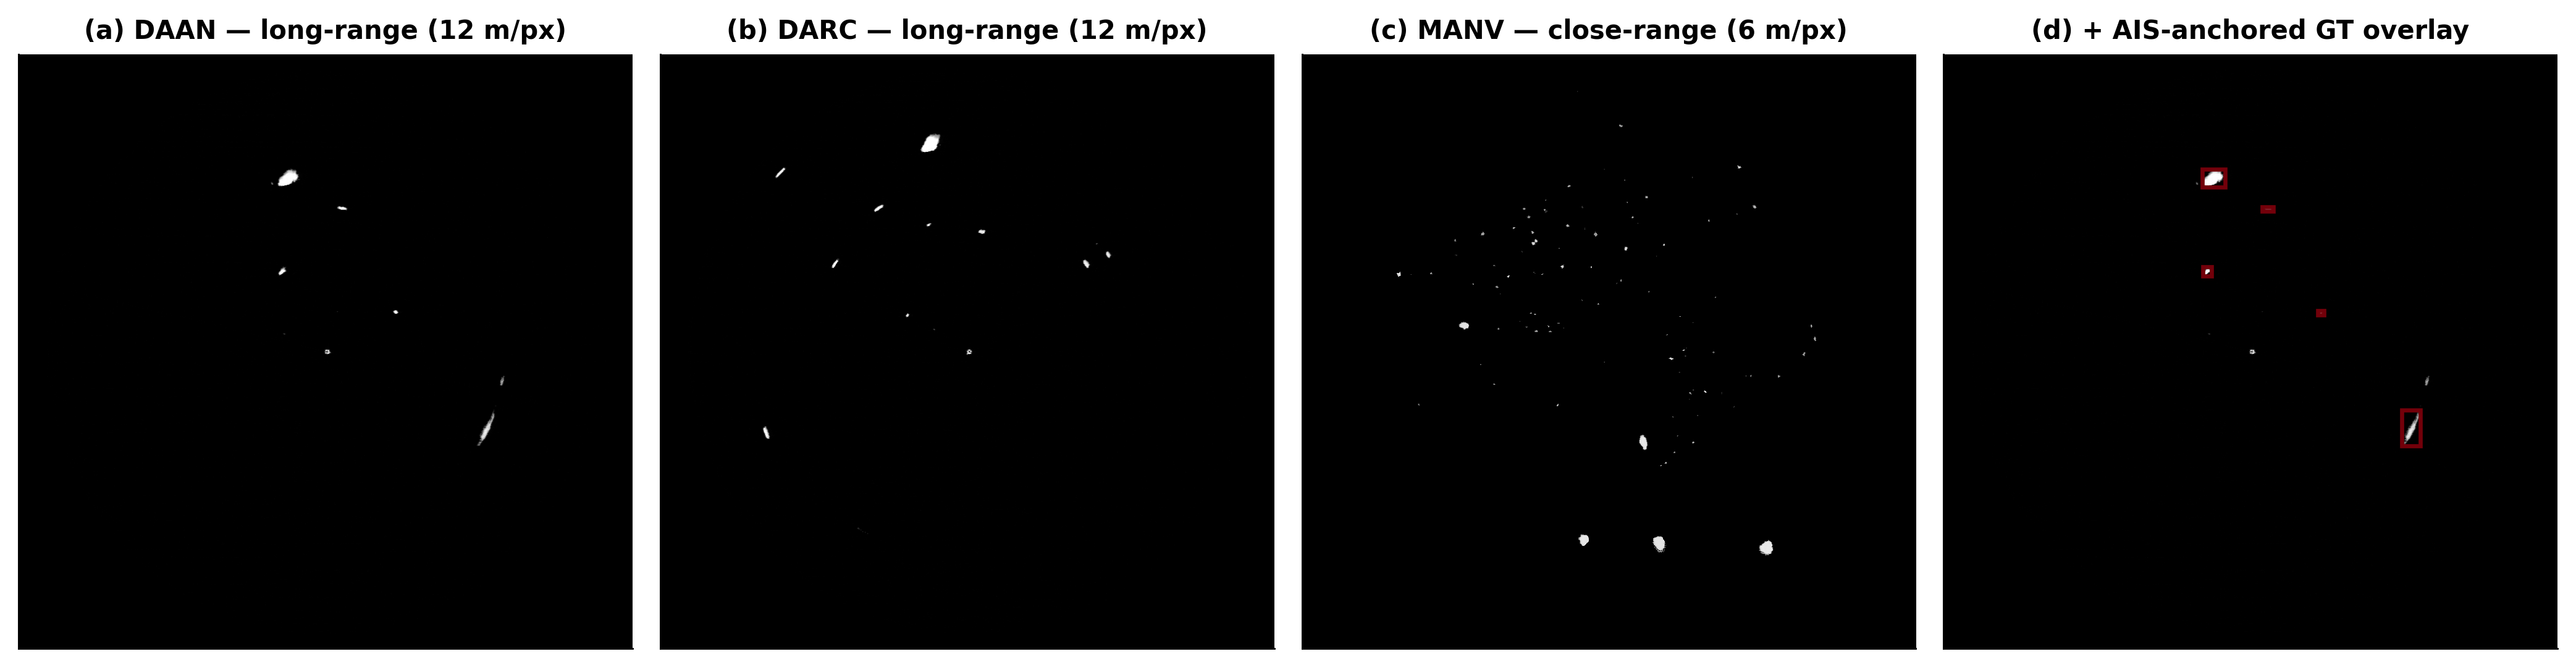
\includegraphics[width=\linewidth]{fig7_preprocess.png}\par
      \sub{Preprocessing: polar PPI $\rightarrow$ masked, calibrated imagery with hybrid AIS-anchored GT boxes.}
  \end{columns}
\end{frame}

% =======================================================================
% 6 Preprocessing contribution (novel)
% =======================================================================
\begin{frame}{Fixing the public DLR release}
  Two systematic issues in the released annotations had to be corrected
  \textbf{before} any detector comparison was meaningful.
  \vspace{0.6em}
  \begin{columns}[T,onlytextwidth]
    \column{0.48\textwidth}
      \begin{block}{1.\ Polar-origin bias (17\,px)}
        Visual PPI centre and polar projection origin were offset by
        \hl{$\sim$17\,px}.  Naive AIS projection placed seeds
        \hl{40--70\,px} from their radar blobs.
        \sub{Fix: separate visual-centre from polar-origin; per-dataset calibration
        reduces residuals to 5--7\,px.}
      \end{block}
    \column{0.48\textwidth}
      \begin{block}{2.\ MANV range-scale error ($2\times$)}
        Published range-per-pixel disagreed with ground truth by a
        factor of two on MANV.  Fit a per-dataset range scale.
        \sub{Fix: dataset-aware calibration of range resolution before projecting AIS tracks into pixel space.}
      \end{block}
  \end{columns}
  \vspace{0.5em}
  \begin{block}{Hybrid AIS-anchored ground truth}
    AIS seeds in pixel space $\rightarrow$ image-grounded connected-component
    refinement $\rightarrow$ tight bounding boxes.  Replaces DBSCAN
    $33\times33$ padded boxes used in prior work.
  \end{block}
\end{frame}

% =======================================================================
% 7 Evaluation protocol
% =======================================================================
\begin{frame}{Evaluation protocol}
  \begin{columns}[T,onlytextwidth]
    \column{0.52\textwidth}
      \begin{itemize}\setlength\itemsep{0.45em}
        \item \hl{COCO suite}: AP@0.50, AP@0.75, AP@[.50:.95], AR@100.
        \item Deep detectors: \hl{three random seeds} (42, 123, 456); report mean $\pm 1\sigma$.
        \item Classical detectors: deterministic; one run per method.
        \item Evaluation surfaces:
          \begin{itemize}\setlength\itemsep{0.15em}
            \item DL --- 4{,}560 tiles of $640\times640$\,px.
            \item Classical --- 760 full PPI frames of $1050\times1024$\,px.
          \end{itemize}
        \item Same AIS-anchored GT geometry on both surfaces.
      \end{itemize}
    \column{0.44\textwidth}
      \begin{block}{Pending analyses (see limitations)}
        \small
        TIDE error decomposition;\\
        pairwise bootstrap significance;\\
        Pareto accuracy-vs-latency curves.
      \end{block}
  \end{columns}
\end{frame}

% =======================================================================
% 8 Main results table
% =======================================================================
\begin{frame}{Main results: DAAN test}
  \centering
  \renewcommand{\arraystretch}{1.12}
  \footnotesize
  \begin{tabular}{@{}l l r r r r@{}}
    \toprule
    \textbf{Method} & \textbf{Type} & \textbf{AP@.50} & \textbf{AP@.75} & \textbf{AP@[.50:.95]} & \textbf{AR@100} \\
    \midrule
    YOLOv11          & DL ($\times3$)   & \textbf{0.776\,\sub{$\pm$.06}} & 0.733\,\sub{$\pm$.04} & 0.610\,\sub{$\pm$.03} & 0.790\,\sub{$\pm$.03} \\
    RT-DETR          & DL ($\times3$)   & 0.738\,\sub{$\pm$.03} & 0.732\,\sub{$\pm$.03} & \textbf{0.635\,\sub{$\pm$.02}} & \textbf{0.876\,\sub{$\pm$.01}} \\
    Faster R-CNN     & DL ($\times3$)   & 0.545\,\sub{$\pm$.04} & 0.533\,\sub{$\pm$.04} & 0.422\,\sub{$\pm$.04} & 0.456\,\sub{$\pm$.04} \\
    \midrule
    Morphological    & Classical        & 0.537 & 0.315 & 0.311 & 0.661 \\
    Otsu             & Classical        & 0.534 & 0.338 & 0.318 & 0.676 \\
    CA-CFAR          & Classical        & 0.483 & 0.408 & 0.388 & 0.832 \\
    SO-CFAR          & Classical        & 0.342 & 0.315 & 0.255 & 0.672 \\
    GO-CFAR          & Classical        & 0.315 & 0.224 & 0.204 & 0.535 \\
    SSOTSU           & Classical        & 0.030 & 0.009 & 0.014 & 0.449 \\
    Wavelet          & Classical        & 0.000 & 0.000 & 0.000 & 0.000 \\
    \bottomrule
  \end{tabular}
  \vspace{0.5em}
  \par\sub{Ranked by AP@0.50. DL columns show mean $\pm 1\sigma$ over 3 seeds.}
\end{frame}

% =======================================================================
% 9 Multi-metric figure
% =======================================================================
\begin{frame}{How the ranking changes across metrics}
  \begin{columns}[T,onlytextwidth]
    \column{0.62\textwidth}
      \centering
      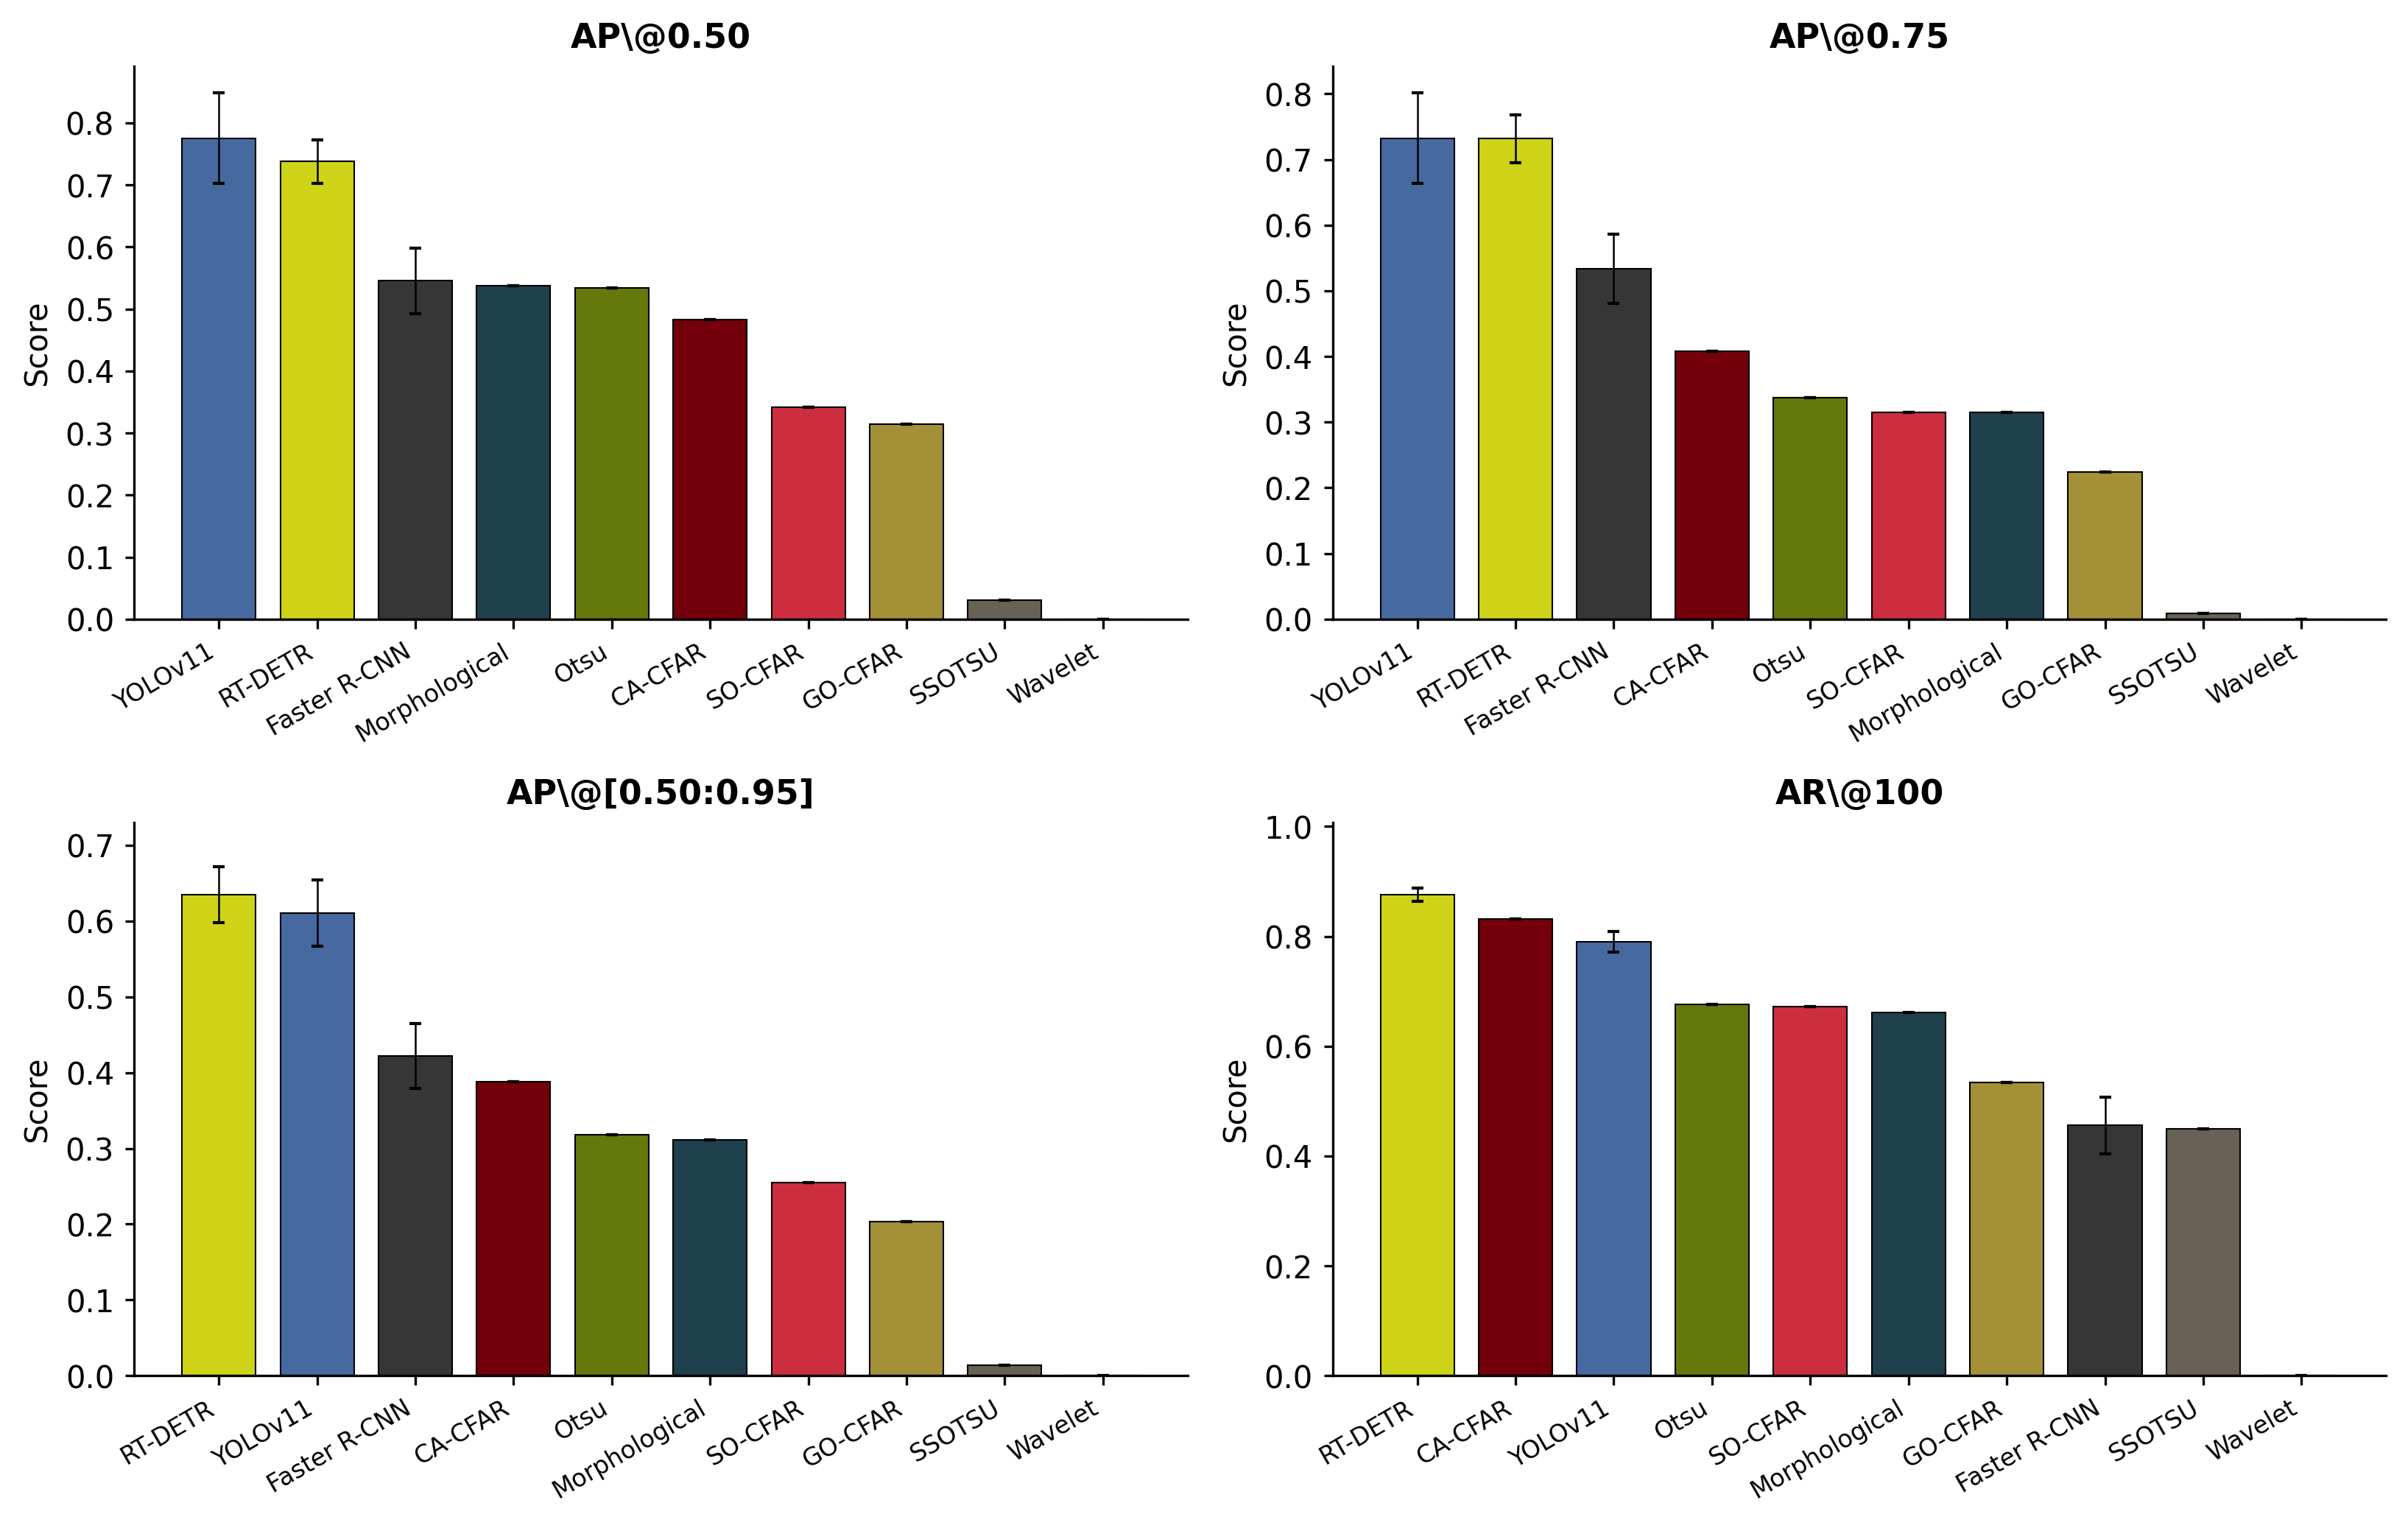
\includegraphics[width=\linewidth]{fig2_multimetric.png}
    \column{0.34\textwidth}
      \begin{itemize}\setlength\itemsep{0.45em}
        \item \hl{YOLOv11} leads AP at every IoU threshold.
        \item \hl{RT-DETR} wins AR@100 --- large prediction volume recovers nearly every target.
        \item \hl{Morphological} and \hl{Otsu} top the classical sub-ranking on precision metrics.
        \item \hl{CA-CFAR} leads classical AR@100: CFAR is fundamentally a strong \emph{recaller}.
      \end{itemize}
  \end{columns}
\end{frame}

% =======================================================================
% 10 Per-dataset inversion (key finding)
% =======================================================================
\begin{frame}{Per-dataset inversion: resolution chooses the detector}
  \begin{columns}[T,onlytextwidth]
    \column{0.58\textwidth}
      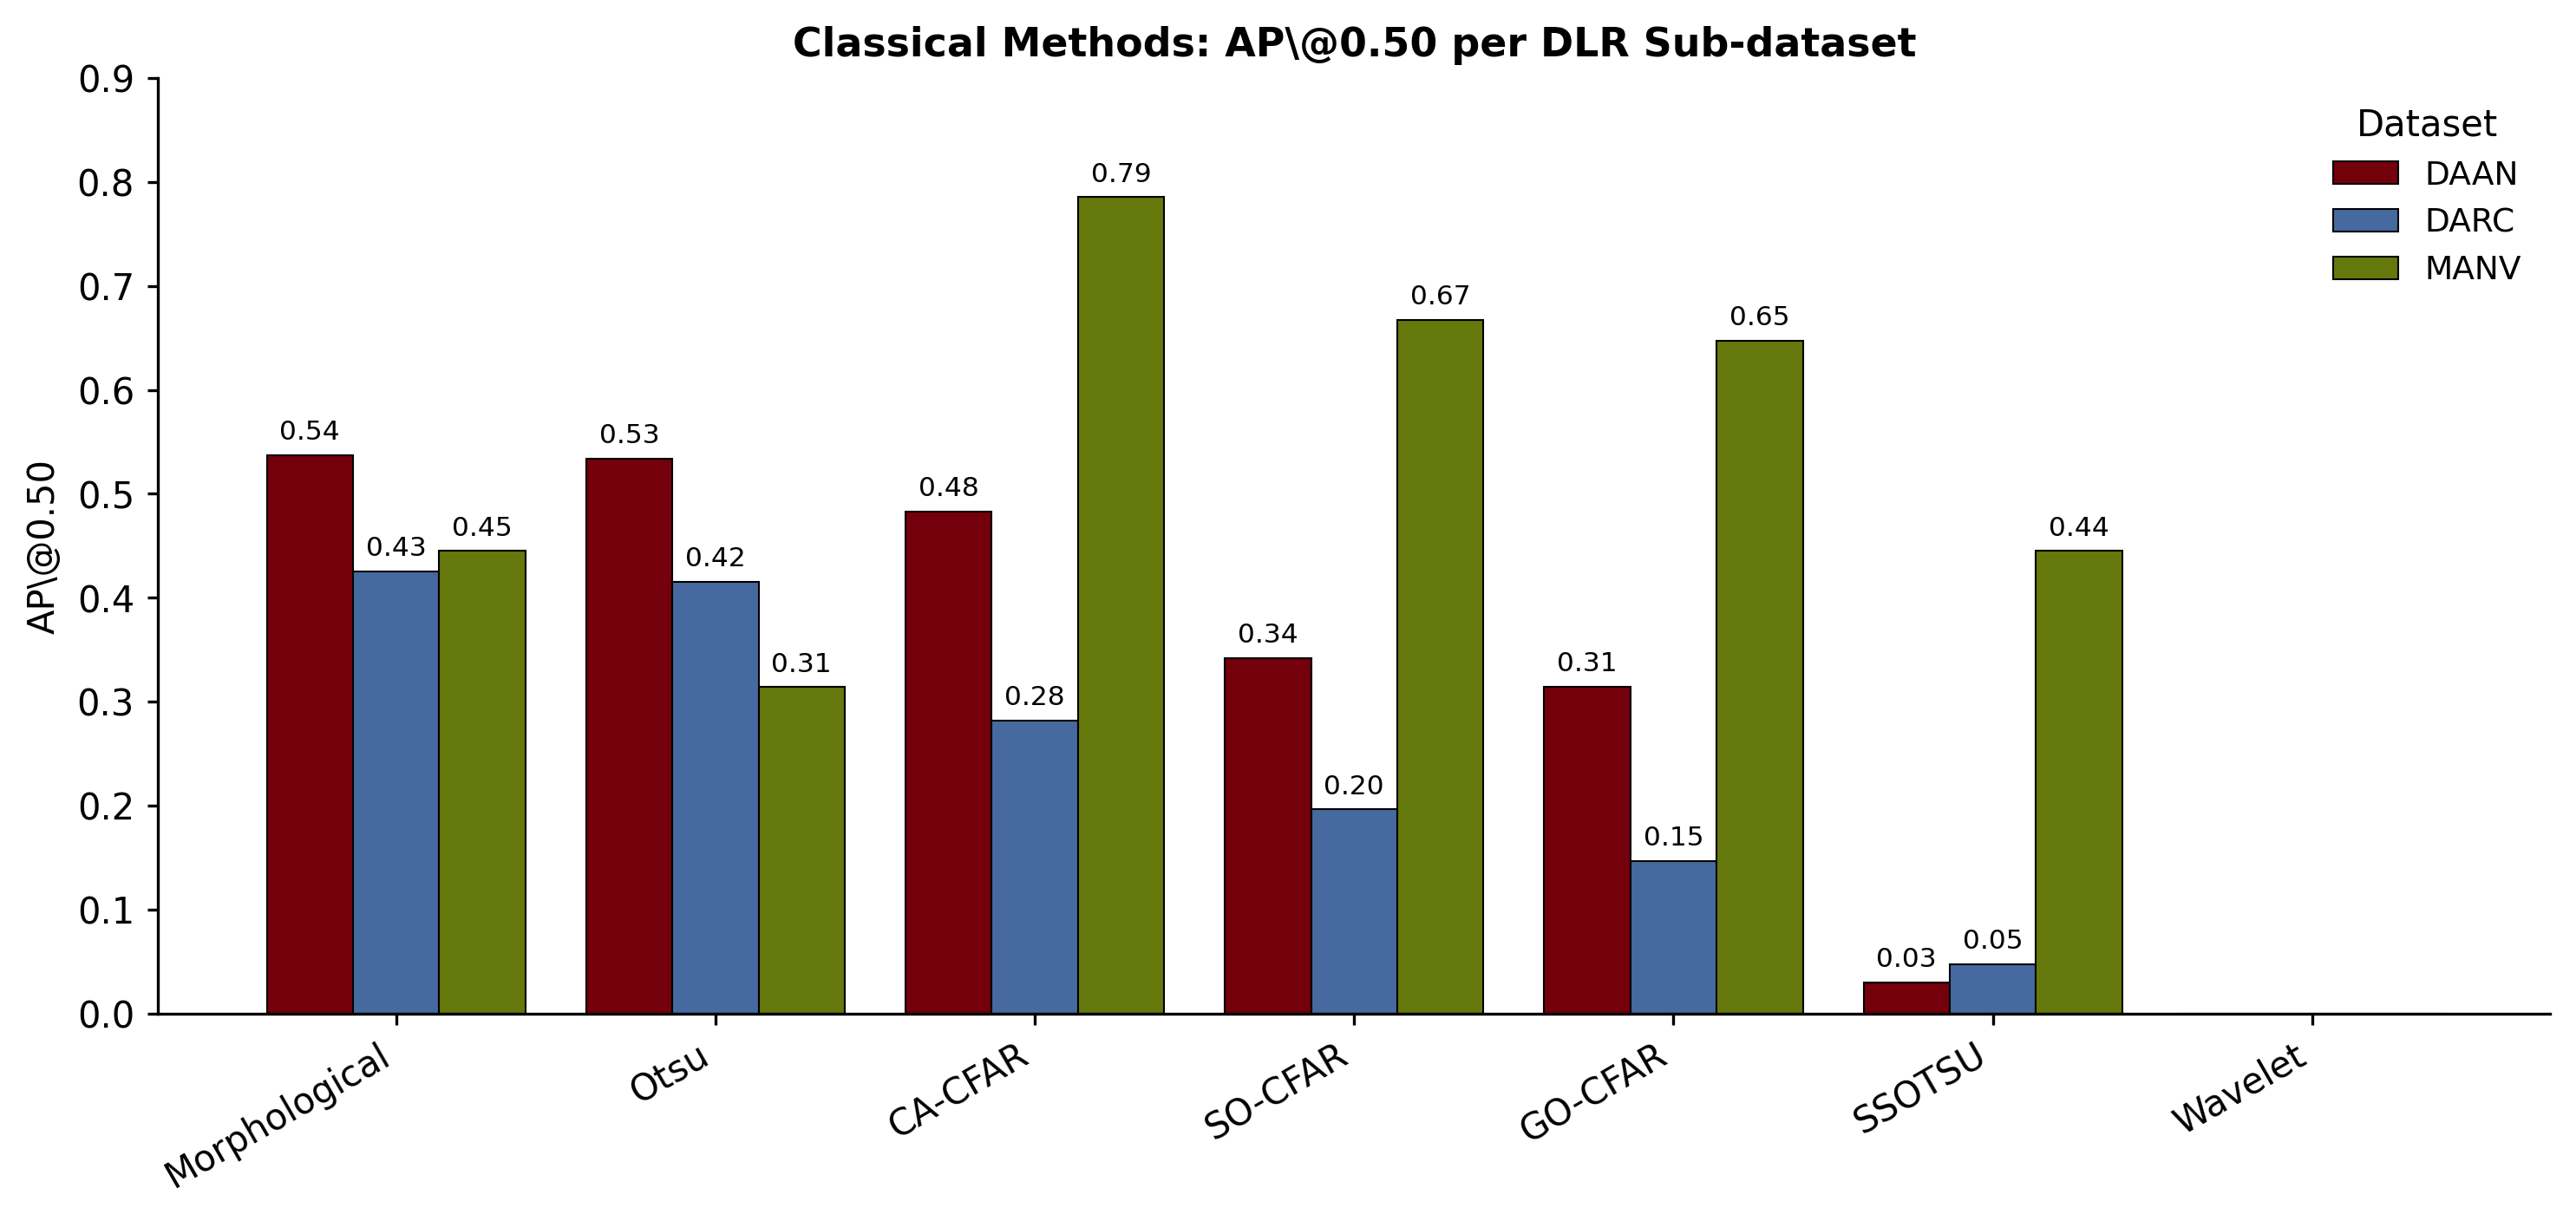
\includegraphics[width=\linewidth]{fig3_per_dataset.png}
    \column{0.40\textwidth}
      \begin{itemize}\setlength\itemsep{0.45em}
        \item On the close-range \hl{MANV} (6\,m/px, harbour),
              \hl{CA-CFAR dominates at AP@0.50 = 0.785}.\\
              \sub{Dense clutter, high-SNR targets, sub-metre cells --- exactly where CFAR was designed to live.}
        \item On long-range \hl{DAAN / DARC} (12\,m/px, open water),
              \hl{morphological / Otsu lead} at 0.53--0.54.
        \item Actionable: \emph{pick the classical detector to match the radar's resolution regime.}
      \end{itemize}
  \end{columns}
\end{frame}

% =======================================================================
% 11 Seed stability
% =======================================================================
\begin{frame}{Deep-learning seed stability}
  \begin{columns}[T,onlytextwidth]
    \column{0.58\textwidth}
      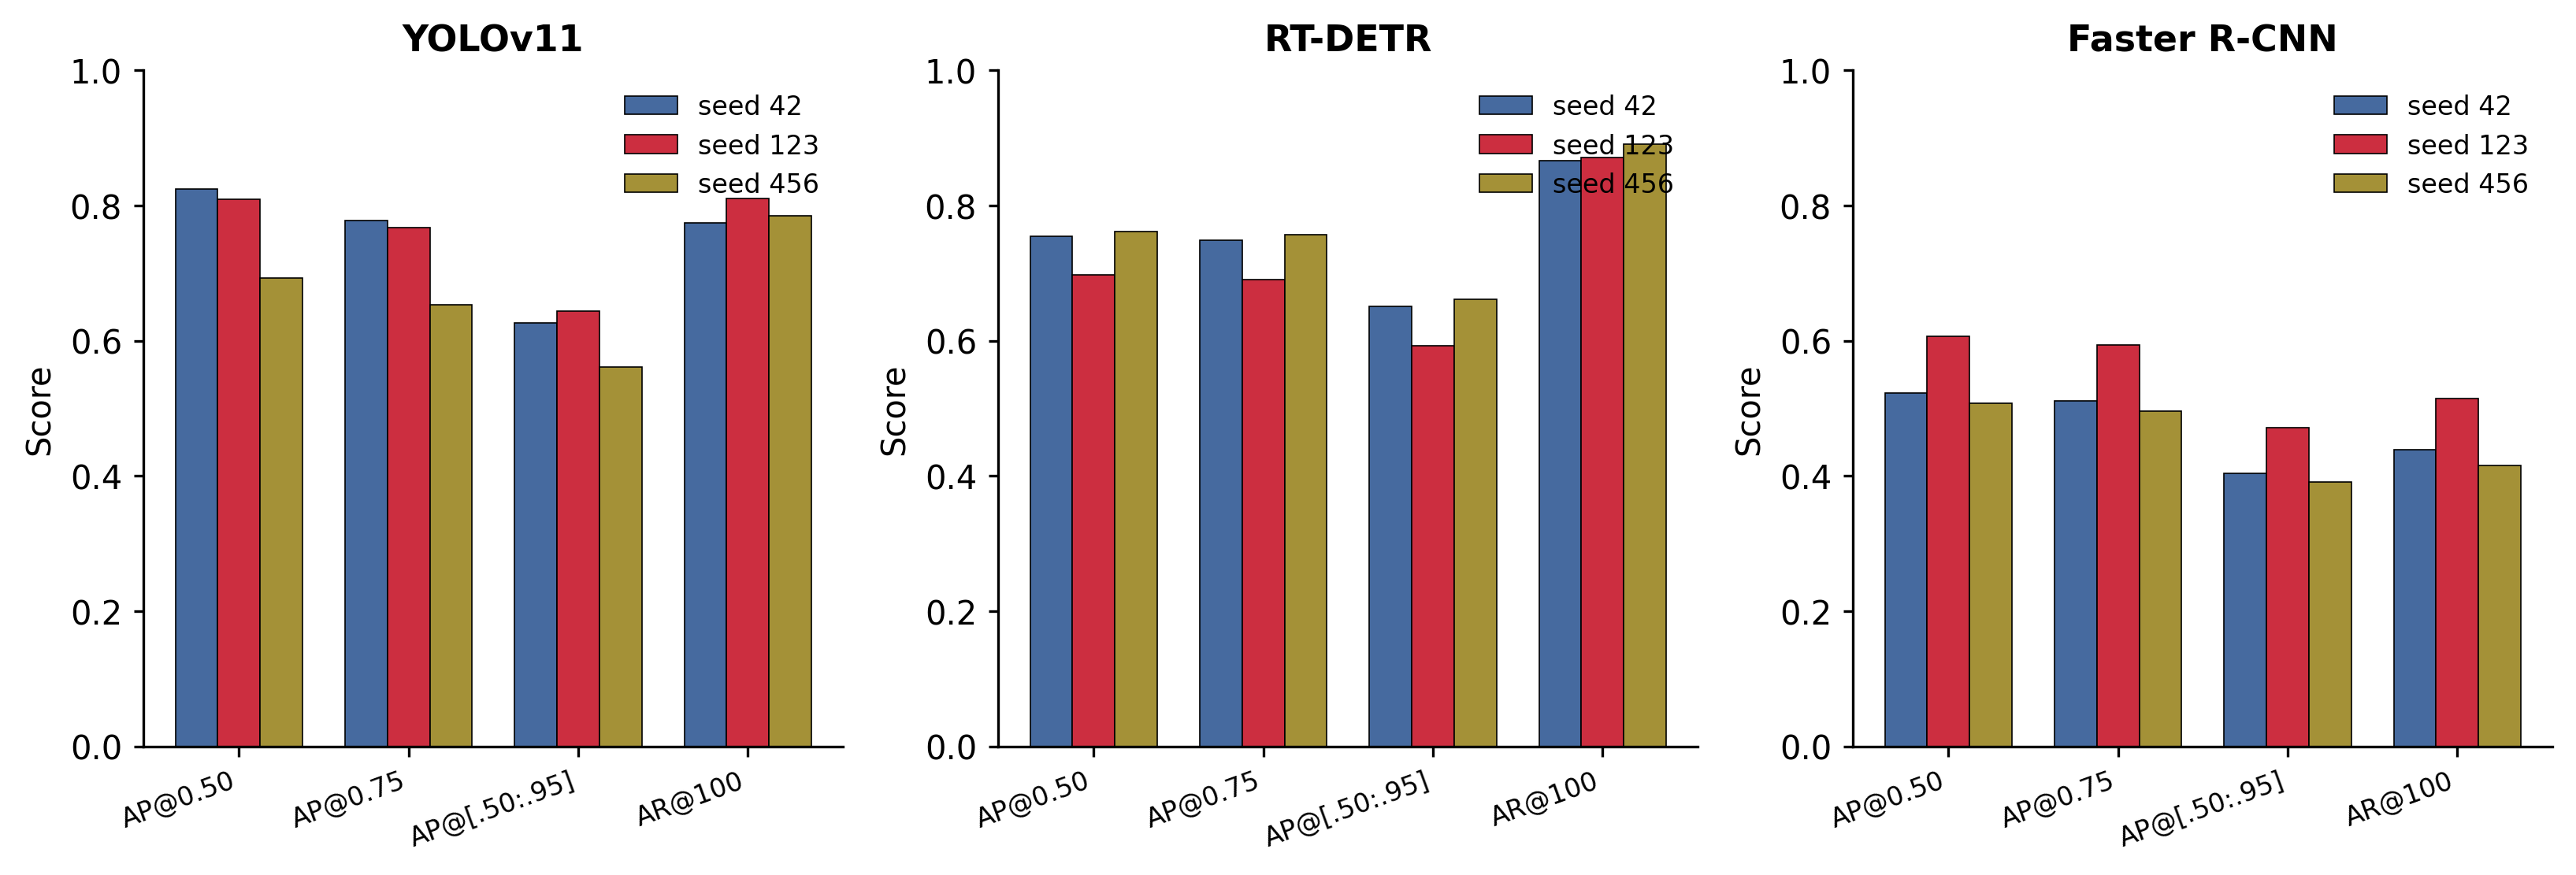
\includegraphics[width=\linewidth]{fig4_dl_seeds.png}
    \column{0.40\textwidth}
      \begin{itemize}\setlength\itemsep{0.45em}
        \item All three DL detectors: $\sigma \le 0.06$ on every metric.
        \item \hl{YOLOv11} is the most consistent ($\sigma\approx 0.01$--$0.02$ on AP).
        \item RT-DETR next; Faster R-CNN most variable.
        \item No seed dominates any single metric $\rightarrow$ the training regime has converged.
      \end{itemize}
  \end{columns}
\end{frame}

% =======================================================================
% 12 Volume vs AP
% =======================================================================
\begin{frame}{Detection volume vs.\ precision}
  \begin{columns}[T,onlytextwidth]
    \column{0.58\textwidth}
      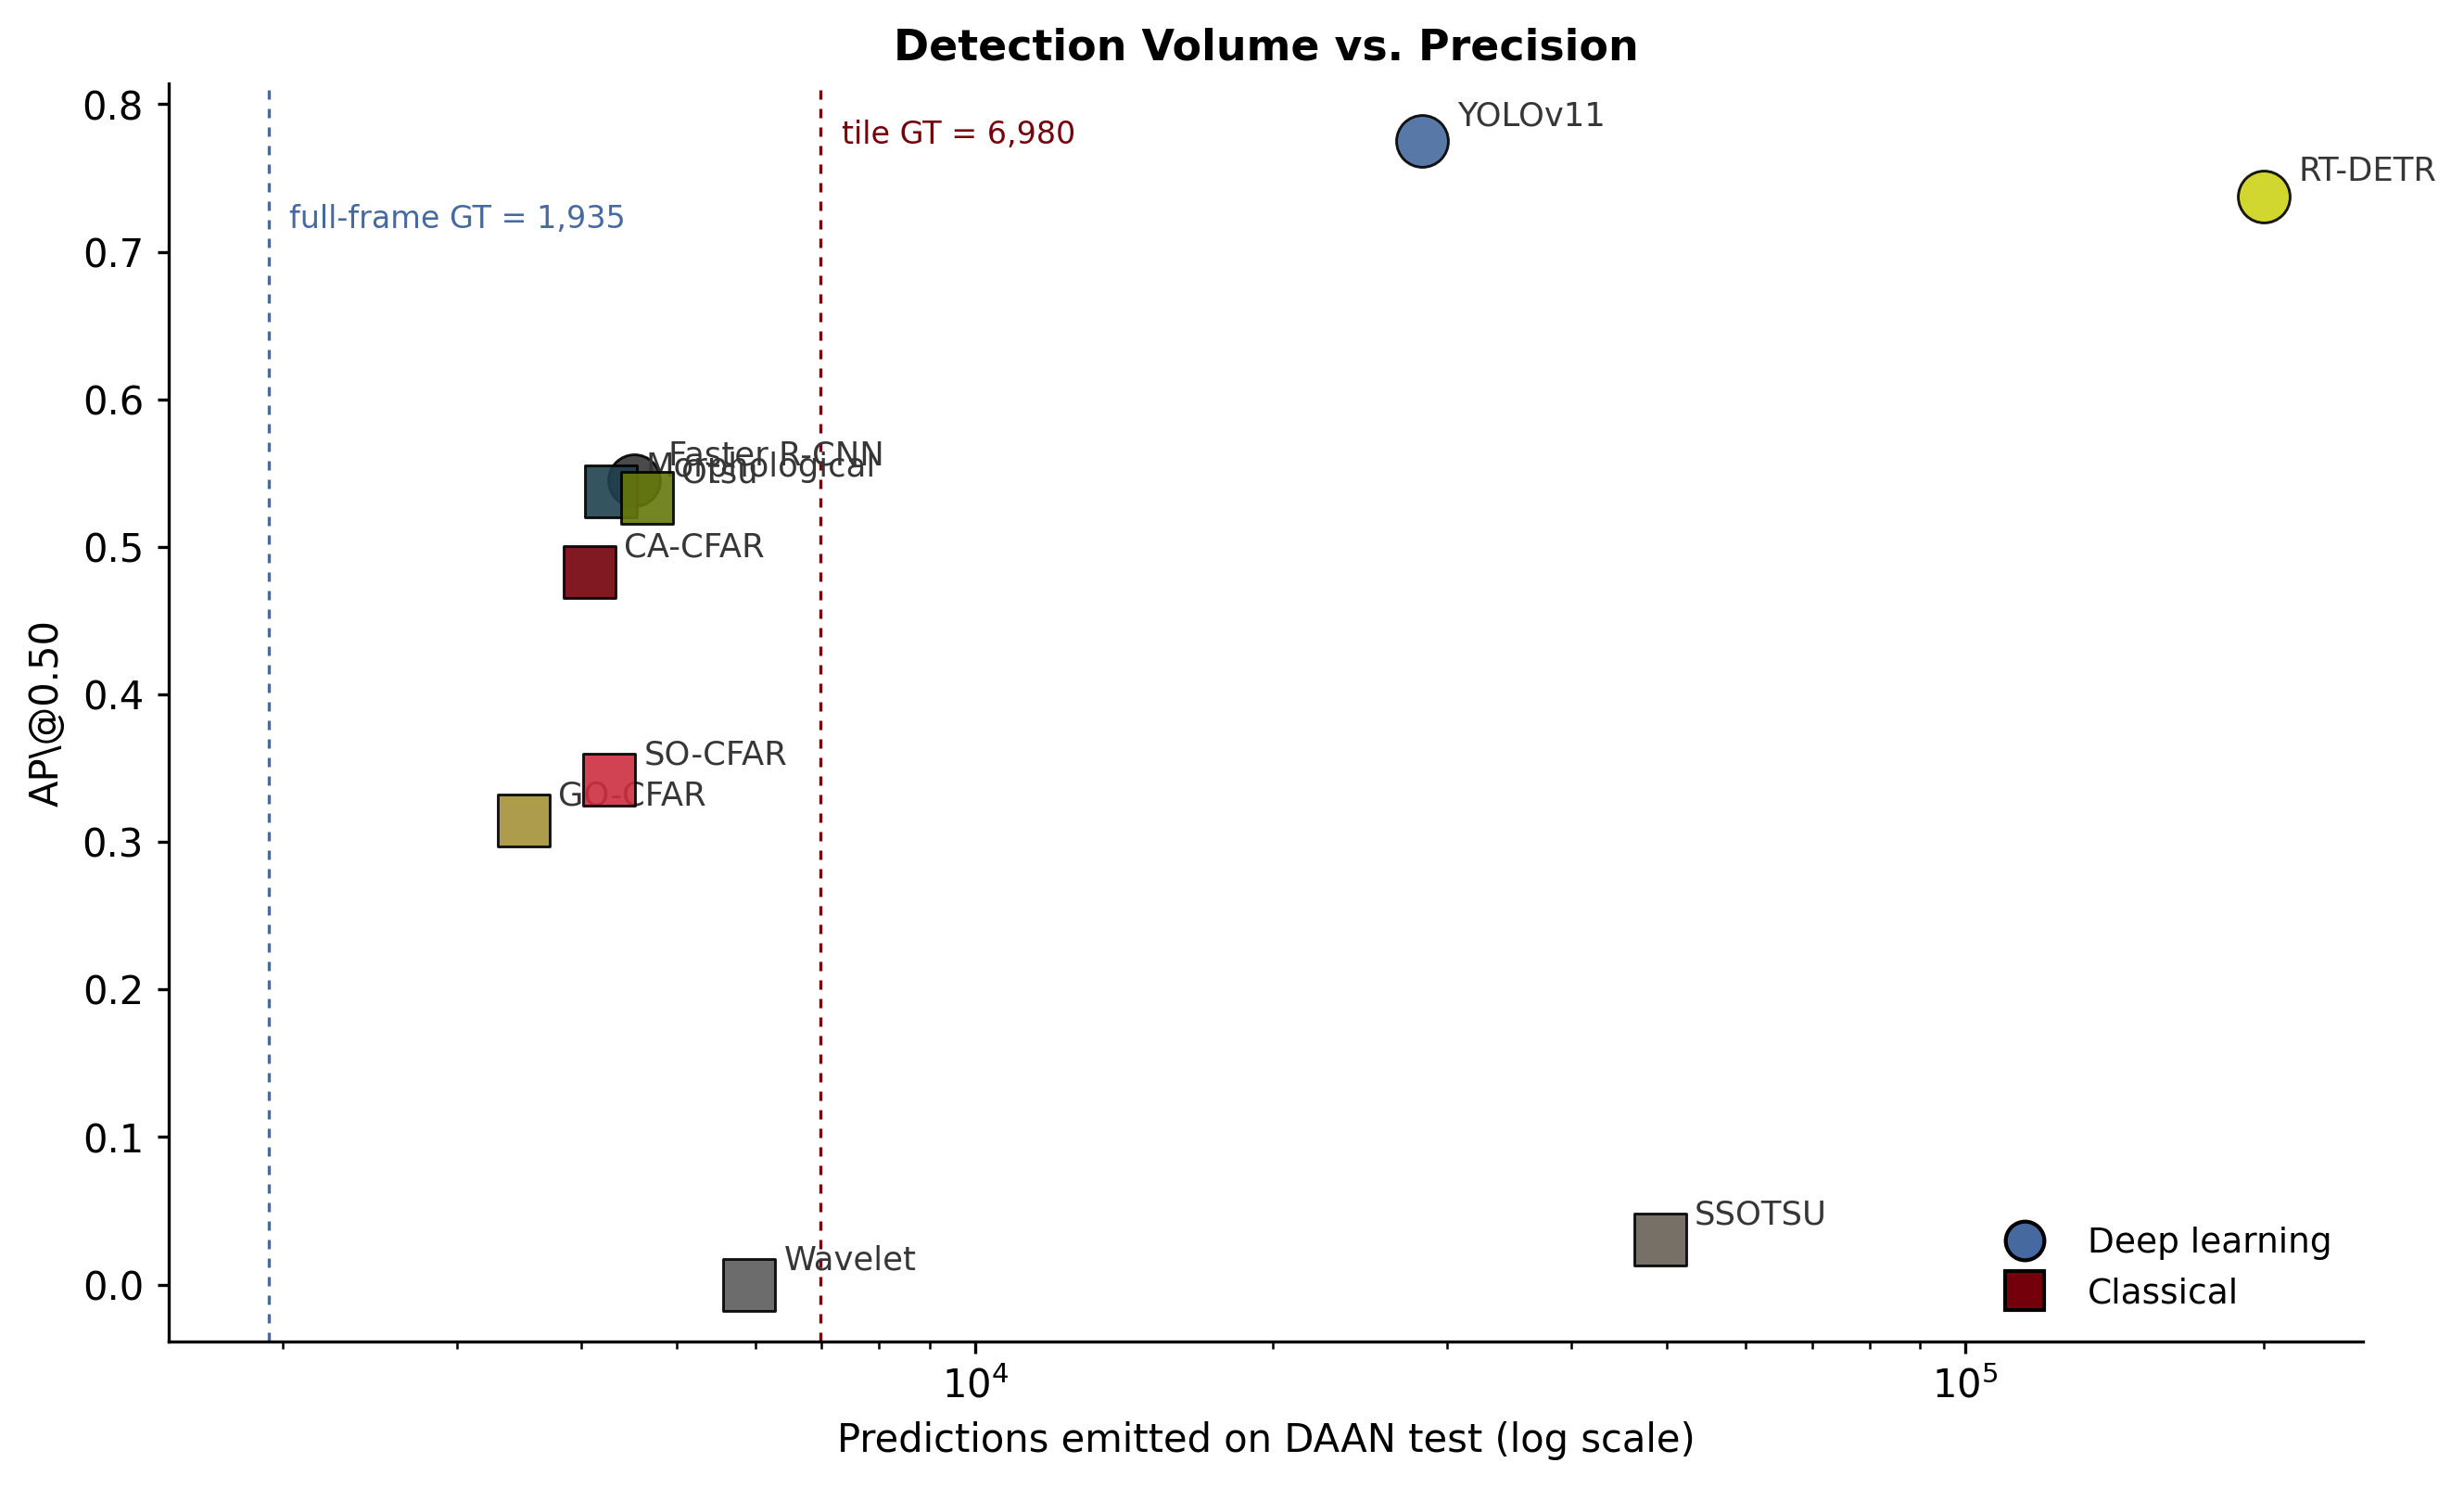
\includegraphics[width=\linewidth]{fig5_count_vs_ap.png}
    \column{0.40\textwidth}
      \begin{itemize}\setlength\itemsep{0.45em}
        \item \hl{Faster R-CNN} --- 4.5\,k preds across 4.56\,k tiles, \emph{one-to-one with tile count}, AP = 0.55.
        \item Classical cluster: 4--8\,k preds, AP = 0.31--0.55.
        \item \hl{RT-DETR} (200\,k) and \hl{YOLOv11} (28\,k) over-predict heavily, but confidence ranking preserves AP.
        \item \hl{SSOTSU} (49\,k / AP 0.03) and \hl{Wavelet} are clear outliers --- both broken at the scoring step.
      \end{itemize}
  \end{columns}
\end{frame}

% =======================================================================
% 13 Discussion
% =======================================================================
\begin{frame}{Takeaways}
  \begin{itemize}\setlength\itemsep{0.55em}
    \item \hl{Deep detectors win the benchmark, but the gap is narrower than the literature implies.}\\
          Best classical (morphological, 0.537) is only \emph{0.008} below Faster R-CNN and reaches \emph{69\%} of YOLOv11 with no training.
    \item \hl{The classical paradigm chooses the detector} at the radar's resolution regime --- CA-CFAR for 6\,m/px, morphological/Otsu for 12\,m/px.
    \item \hl{Why our numbers sit below published results} (e.g.\ YOLOv11 0.776 vs reported 0.95): prior work matches against DBSCAN-padded $33\times33$ boxes.  We use \emph{tight} AIS-anchored GT --- harder, but operationally predictive.
  \end{itemize}
\end{frame}

% =======================================================================
% 14 Limitations / remaining work
% =======================================================================
\begin{frame}{Limitations and remaining work}
  \begin{columns}[T,onlytextwidth]
    \column{0.48\textwidth}
      \begin{block}{Known failures}
        \small
        \begin{itemize}\setlength\itemsep{0.25em}
          \item \hl{Wavelet-SWT}: 44$\times$47\,px blobs vs GT 15$\times$15 $\rightarrow$ AP = 0.
          \item \hl{SSOTSU}: 49\,k over-predictions $\rightarrow$ AP = 0.03.
          \item \hl{U-Net}: training did not finish in time for this draft.
          \item \hl{OS-CFAR}: coded, not yet reported.
        \end{itemize}
      \end{block}
    \column{0.48\textwidth}
      \begin{block}{Pending proposal deliverables}
        \small
        \begin{itemize}\setlength\itemsep{0.25em}
          \item TIDE error decomposition (classification / localization / background / duplicate / missed).
          \item Pairwise bootstrap significance (10\,000 resamples, Bonferroni).
          \item Accuracy-vs-latency Pareto (FLOPs, inference time, parameter count).
          \item Per-size AP stratification (APs / APm / APl).
          \item YOLOv11-OBB + SAHI re-run.
        \end{itemize}
      \end{block}
  \end{columns}
\end{frame}

% =======================================================================
% 15 Conclusion
% =======================================================================
\begin{frame}{Conclusion}
  \begin{itemize}\setlength\itemsep{0.55em}
    \item First controlled cross-paradigm benchmark of \hl{7 classical + 4 deep} detectors on X-band marine radar PPI.
    \item Two systematic flaws in the public DLR release corrected:
          \hl{17-px polar-origin bias} and \hl{2$\times$ MANV range-scale error}.
    \item Hybrid AIS-anchored / image-grounded GT generator released.
    \item Under the cleaner evaluation: YOLOv11 leads at \hl{0.776 $\pm$ 0.06},
          RT-DETR 0.738, Faster R-CNN 0.545; classical competitive but below, with \hl{CA-CFAR 0.785 on MANV}.
  \end{itemize}
  \vspace{0.4em}
  \begin{center}
    {\color{garnet}\rule{0.8\textwidth}{0.6pt}}\par
    \vspace{0.3em}
    \small All code, configs, checkpoints, calibration, and GT generator released.\\
    \small \texttt{github.com/j-vaught/marine-radar-detection}
  \end{center}
\end{frame}

\end{document}
